\documentclass[11pt]{article}
\usepackage[pdftex]{graphicx}

\usepackage{henrian-basic}
\usepackage{henrian-homework}
\usepackage{chngpage}

\usepackage{amsmath}
\usepackage{float}
\usepackage{natbib}
\bibliographystyle{plainnat}
\bibpunct{(}{)}{,}{a}{,}{,}

\makeHeaders{Machine Learning: Homework 8}

\begin{document}

\begin{itemize}
  \item \textbf{Email}: chrisbrown@utexas.edu
  \item \textbf{EID}: chb595
\end{itemize}

\section{Genetic Algorithms}

\subsection{My algorithm}




\subsection{Crossover}
The intution behind crossover is that if you take two strings that 

I tried various versions of crossover; for two strings A and B:
\begin{enumerate}[a.]
  \item One cut:
    \[
      \frac{abcd\mathbf{ef}}{zyxw\mathbf{vu}} \to \frac{abcd\mathbf{vu}}{zyxw\mathbf{ef}}
    \]
  \item Two cuts:
    \[
      \frac{ab\mathbf{cd}ef}{zy\mathbf{xw}vu} \to \frac{ab\mathbf{xw}ef}{zy\mathbf{cd}vu}
    \]
  \item Two cuts per string:
    \[
      \frac{ab\mathbf{cde}f}{zy\mathbf{x}wvu} \to \frac{ab\mathbf{x}ef}{zy\mathbf{cde}wvu}
    \]
\end{enumerate}
I did not formally compare the different approaches, but the last seemed to work the best. (a) and (b) are basically the same; picture the sequence of pairs of indices as a ring, and it becomes clear that (a) is just (b) while setting the second cut to the end of the string, as noted by \citet{whitley:1993}, who credits this observation to \citet{dejong:1975}.

The alternative, (c), is even more flexible than (b), by which I mean that it will generate more variety. A string of one swap could become a string of two in one crossover. While this is unnatural when considered in the context of biological crossover, it seems more suitable here because it is a generalization of (b), and we want to try out as many different combinations as possible, as quickly as possible. The human genome is not functionally homogenous; the first percent and the last percent most likely correspond to very different operations. But each swap in the sequence we consider in this problem is the same operation. Certainly, the order of swaps matters, but not as much as in a complex biological genome.

\subsection{Mutation}
Mutation is simpler than crossover; in my implementation, there is one parameter that determines the probability that we will mutate a given candidate in a particular generation. I take the simplest route; with a constant probability $p_{mutation}$, I replace one swap in a candidate, chosen by random, with a completely random new swap. There are variations; we could also specify how many mutations to execute, but the same effect is achieved over several generations by simply choosing a different $p_{mutation}$. Or we could mutate a swap by only changing only one of the indices, or by changing the indices by only a small amount. However, I only implemented the simplest approach, where I fully replace one swap with an entirely random new pair of indices.

\section{Results}

In Figure \ref{fig:best-solution-performance}, you can see the best solution's performance, plotted as the number of generations progresses. As you can see, it converges pretty quickly---it took just over 600 generations.

\begin{figure}[H]
  \centering
  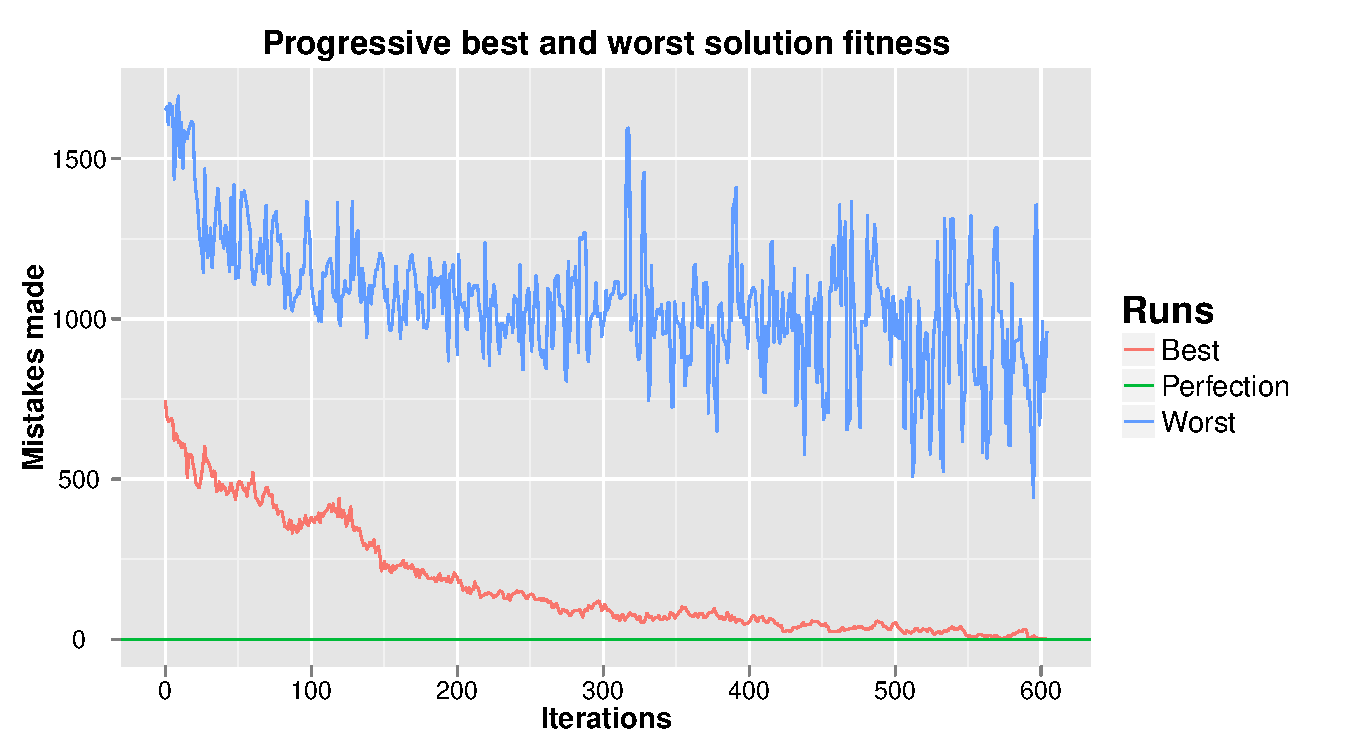
\includegraphics[width=0.95\textwidth]{results/output-i600-fitness.pdf}
  \caption{The best solution's performance, over generation. Lower is better, because my fitness function measured mistakes made in ordering.}
  \label{fig:best-solution-performance}
\end{figure}

\noindent
And in Figure \ref{fig:best-solution-length}, I show see the length of the best solution, plotted against the number of generations elapsed.

\begin{figure}[H]
  \centering
  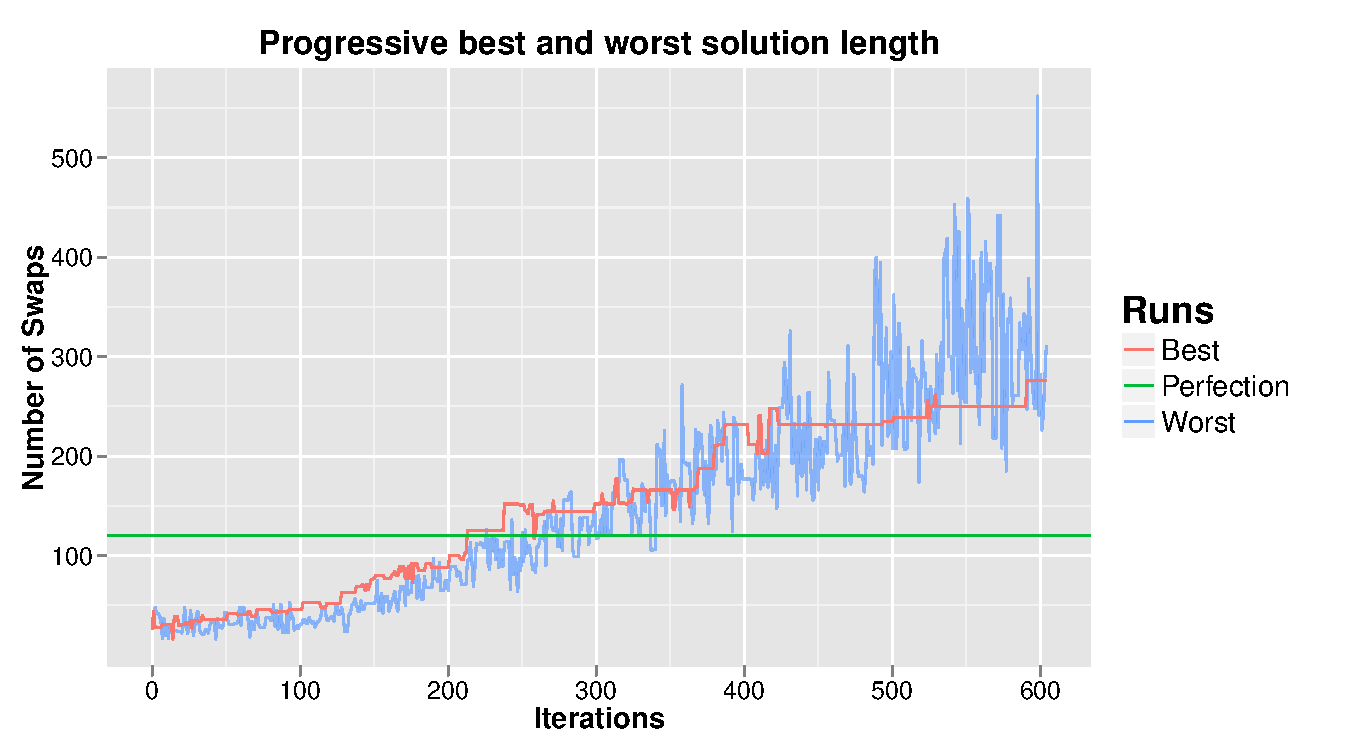
\includegraphics[width=0.95\textwidth]{results/output-i600-length.pdf}
  \caption{The best solution's length, over generation.}
  \label{fig:best-solution-length}
\end{figure}

\subsection{Solution}

Here is a final solution, a final parasite sequence, and the solution's sort of that sequence:

\begin{figure}[H]
  \begin{adjustwidth}{.5in}{.5in}
    \begin{footnotesize}
      (2,13) (2,2) (7,3) (8,4) (4,2) (7,14) (9,10) (12,7) (2,2) (11,2) (9,14) (4,12) (13,2) (7,4) (5,9) (2,2) (5,5) (4,2) (7,14) (8,7) (9,11) (15,5) (12,12) (11,13) (10,11) (10,7) (12,7) (1,9) (9,10) (7,4) (9,11) (15,5) (12,12) (12,7) (5,9) (4,12) (6,5) (2,9) (7,8) (7,3) (10,14) (7,14) (7,8) (4,12) (9,10) (2,15) (8,0) (3,14) (1,12) (8,6) (12,7) (6,15) (5,9) (15,2) (2,9) (4,12) (9,10) (2,15) (8,0) (3,14) (1,12) (8,6) (12,7) (6,15) (12,7) (1,7) (14,11) (9,10) (15,11) (6,7) (10,7) (7,3) (11,3) (15,5) (2,2) (7,14) (9,10) (15,2) (10,11) (11,3) (7,8) (15,12) (9,3) (2,9) (6,9) (6,7) (15,12) (9,3) (12,7) (2,9) (10,11) (7,8) (7,8) (7,4) (5,9) (12,12) (2,15) (8,0) (7,4) (5,9) (2,2) (7,3) (8,4) (4,2) (7,14) (9,10) (12,7) (2,2) (5,5) (9,14) (4,12) (10,14) (7,14) (7,8) (4,12) (9,10) (2,15) (8,0) (3,14) (1,12) (8,6) (5,9) (15,2) (6,7) (12,7) (12,7) (6,15) (6,15) (5,9) (1,12) (8,6) (12,7) (6,15) (5,9) (15,2) (14,0) (13,2) (7,4) (5,9) (2,2) (5,5) (6,7) (10,7) (7,3) (9,10) (12,12) (15,2) (9,10) (2,9) (10,11) (7,8) (15,12) (9,3) (12,7) (15,2) (9,10) (11,5) (10,11) (7,8) (15,12) (11,3) (12,7) (5,9) (2,2) (6,9) (7,8) (11,13) (10,11) (9,11) (3,14) (1,12) (8,6) (13,0) (6,15) (5,9) (15,2) (14,0) (13,2) (7,4) (5,9) (2,2) (5,5) (4,2) (7,14) (8,7) (9,11) (15,5) (12,12) (11,13) (10,11) (10,7) (12,7) (1,9) (9,10) (7,4) (9,11) (15,5) (12,12) (12,7) (5,9) (4,12) (6,5) (2,9) (7,8) (7,3) (10,14) (7,14) (7,8) (4,12) (9,10) (2,15) (8,0) (3,14) (1,12) (8,6) (12,7) (6,15) (5,9) (15,2) (14,0) (13,2) (7,4) (5,9) (2,2) (5,5) (4,2) (7,14) (8,7) (9,11) (15,5) (12,12) (11,13) (10,11) (10,7) (12,7) (1,7) (15,11) (6,7) (10,7) (7,3) (11,3) (15,5) (2,2) (12,12) (2,13) (7,8) (15,12) (11,13) (10,11) (10,7) (7,3) (4,12) (12,12) (15,2) (9,10) (2,9) (10,11) (9,10) (1,2) (2,13) (12,12) (15,2) (9,10) (2,9) (10,11) (7,8) (15,12) (9,3) (12,7) (9,11) (0,15) (0,0) (13,14) (1,15) (3,12) (8,10)
    \end{footnotesize}
  \end{adjustwidth}
  \caption{The final solution. Total length: 276.}
\end{figure}

\begin{figure}[H]
  \begin{small}
    \begin{center}
      \begin{tabular}{rcccccccccccccccc}
        Parasite: & 59 & 80 & 81 & 41 & 88 & 83 & 56 & 76 & 92 & 62 & 19 & 98 & 98 & 69 & 91 & 55 \\
        Solution: & 19 & 41 & 55 & 56 & 59 & 62 & 69 & 76 & 80 & 81 & 83 & 88 & 91 & 92 & 98 & 98 \\
      \end{tabular}
    \end{center}
  \end{small}
  \caption{A sort by the final solution of one of the most difficult parasites.}
\end{figure}

\bibliography{/Volumes/Zooey/Dropbox/ut/tex/liography}

\end{document}

% The final homework is posted and due Tuesday April 24 at 11:59pm. You may use Python or Java if you prefer.
